%!TEX encoding=UTF-8 Unicode
%!TEX root=../tabarnac.tex

\section{Related Work}
\label{sec:soa}

This section presents an overview of related work in the area of memory access
profiling for parallel applications based on shared memory.
We also discuss some mechanisms to improve performance on NUMA architectures.

\subsection{Memory Profiling}
\label{sec:soa-profiling}

Generic tools to evaluate parallel application performance, such as Intel's
VTune~\cite{Reinders05VTune} and Performance Counter
Monitor~(PCM)~\cite{Intel2012b}, the HPCToolkit~\cite{Adhianto10HPCTOOLKIT},
and AMD's CodeAnalyst~\cite{Drongowski2008}, provide only indirect information
about the memory access behavior, more specific tools are therefore required to improve it.

Profiling memory behavior raise two major challenges.
The first one is the collection of accurate and detailed information: performance counters provide precise and easy access to statistics about the CPU usage, but there are few such mechanisms for the memory.
For a maximum level of detail, memory access traces need to be created.
The second challenge is the amount of information that needs to be interpreted and presented to the developer.
Memory access traces provide huge amounts of information on several
dimensions: data structure, threads, access type (read/write), sharing, time of access.
Presenting them to the developer in a readable and meaningful way is therefore not trivial.

\subsubsection{Data Collection}

Several methods have been used to address the problem of data collection. A
lot of studies deduce information from hardware performance
counters~\cite{Majo13(Mis)understanding,
Jiang14Understanding,Bosch00Rivet,Weyers14Visualization,Tao01Visualizing,DeRose01Hardware},
which are special registers that allow to record events such as cache misses and remote
memory accesses. However, these counters only provide a partial
view of the execution, they show events happening on the processor related to
memory, but not what triggered them. Moreover, most available performance counters
depend on the architecture, therefore it is hard to reproduce the same
analysis on different machines with these tools.


Another approach used by several
tools~\cite{Lachaize12MemProf,McCurdy2010,Liu14Tool,Gimenez14Dissecting}
consists of using sampling mechanisms such as AMD's Instruction Based Sampling
(IBS)~\cite{Drongowski07Instructionbased} or Intel Precise Event Based
Sampling (PEBS) to analyze applications. Not only can sampling miss important events, leading to
inaccurate characterizations, but these technologies are usually not portable and work
only with a few recent architecture, therefore such tools can only be used in
special circumstances.

Other studies uses hardware modification (with or without simulation)~\cite{Bao08HMTT,Martonosi92MemSpy}.
Although they provide more efficient trace collection than tools implemented purely in software, they are even less portable.
Finally, binary instrumentation can provide information about memory access behavior~\cite{DeRose02SIGMA}, although this method is slower than
the other previously described, it is more portable and precise. Moreover, as
we show in Section~\ref{sec:expe-overhead}, an efficient instrumentation can
provide an acceptable overhead.

\subsubsection{Visualization}

The second difficulty of memory analysis is to present the information in such
a way that the developer can use it to improve the application. Some of the tools
previously mentioned only provide a textual
output~\cite{Lachaize12MemProf,McCurdy2010,Martonosi92MemSpy}. Even if these
tools highlight the most relevant informations, it is hard to get an overview
of the memory behavior from such output. The developer might be faced with a huge
amount of information and not be able to differentiate normal behaviors from
problematic ones.


Other tools provide more advanced visualizations. For
instance, Tao et al.~\cite{Tao01Visualizing} propose a detailed view of each memory
page, showing the number of remote and local accesses from each NUMA node. Weyers et
al.~\cite{Weyers14Visualization} depict the memory bandwidth between each pair of nodes,
showing where the remote accesses occur. Other
tools~\cite{DeRose01Hardware,DeRose02SIGMA,Bosch00Rivet} provide several views
of the execution, giving the ability to correlate them with the source code of applications, similar to traditional performance tools such as Vtune. Although
all these tools can help developers understand the kind of
performance issues they are facing, they never give the reason \emph{why} a particular
issue is happening, for instance by showing the distribution of memory accesses within data structures.

\begin{figure}[htb]
    \centering
    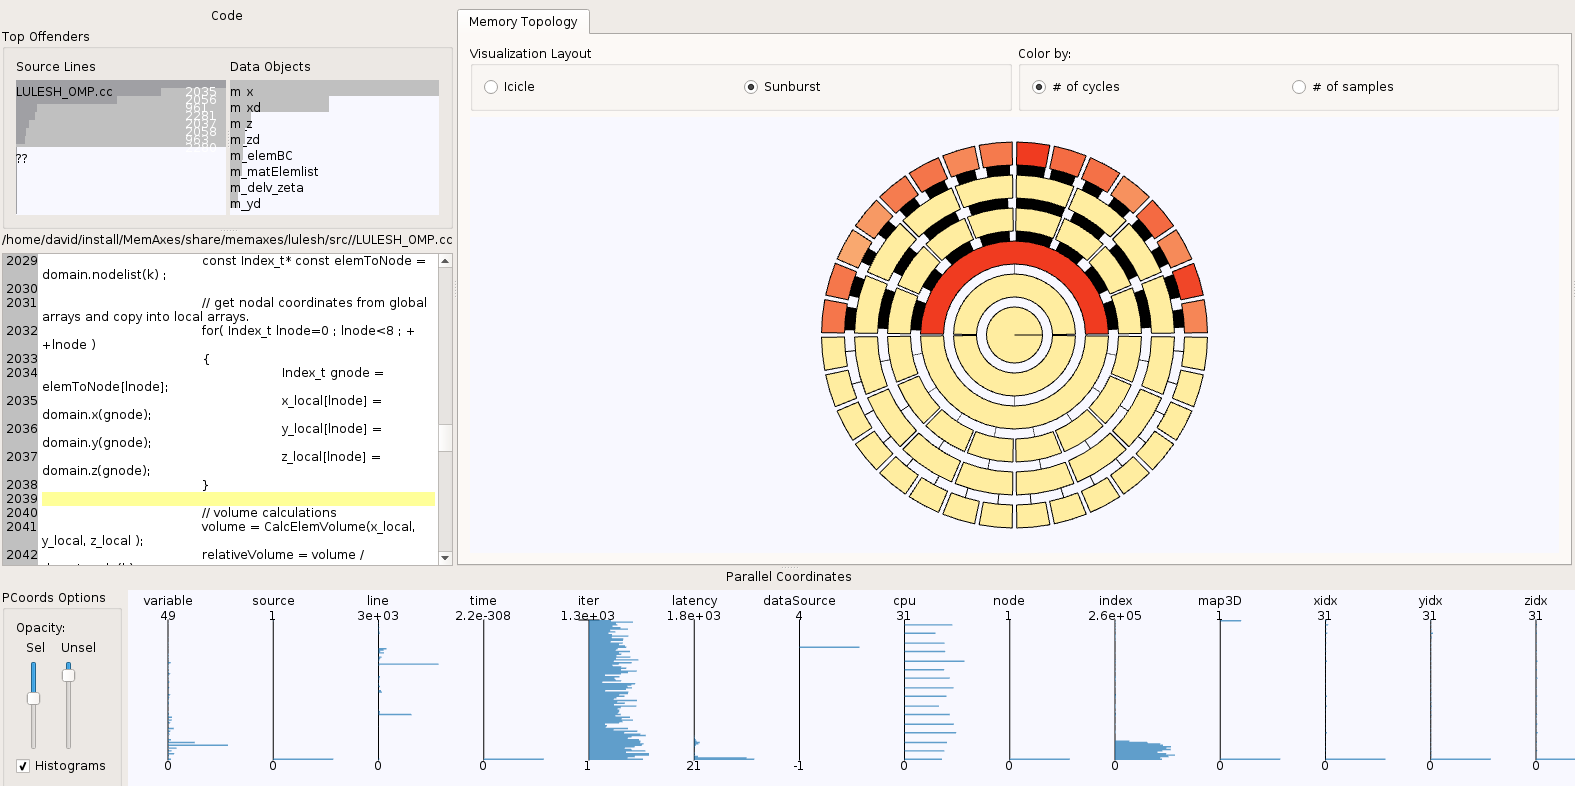
\includegraphics[width=\linewidth]{memAxes.png}
    \caption{Screenshot from MemAxes on the example data trace provided with the
    tool.}
    \label{fig:memaxes}
\end{figure}

MemAxes~\cite{Gimenez14Dissecting} is one of the most advanced NUMA-oriented
visualization tools.
Figure~\ref{fig:memaxes} shows a screenshot of this tool on an example
trace. It shows the source code of the
application (left upper side), the NUMA hierarchy of the machine (right upper side)
and a \emph{parallel coordinate graph} (lower side) designed to help correlating information.
Although this visualization is designed to help understanding NUMA performance
issues, it shows \emph{which} event occurs and \emph{where} it occurs, but does not
tell directly \emph{why} it occurs. The user still has to correlate several pieces of
information to guess the source of a performance issue.

Finally, the proposal of Liu et al.~\cite{Liu14Tool} is quite similar to the previous studies, but
they also provide an \emph{address centric} visualization, which shows how
much each thread accesses a data structure. Such a visualization is a bit closer
to providing the source of the performance issue, but it does not show how the
accesses are distributed inside a structure, and how the structure is shared between
the threads.

%Previous studies aimed to answer this question for some specific
%benchmarks~\cite{Majo13(Mis)understanding,Jiang14Understanding}.
%However, these studies use manual source code analysis and performance counters and do not provide a general tool or methodology that is usable for other applications.
\subsection{Data Mapping Mechanisms}
\label{sec:soa-mapping}

%From a high-level view, data mapping mechanisms can be classified into two categories.
%Mechanisms that have information about the memory accesses before the application starts executing, and mechanisms without prior information that need to determine the memory access behavior during execution of the parallel application.
% There are two kinds of data mapping mechanisms: the ones which have prior
% information about the memory accesses and the ones which do not. The formers can
% have higher improvements, as the collection of information induce a
% potentially high overhead, limiting the quantity and accuracy of information that can be collected.
% But the others do not require any prior analysis.
%Furthermore, opportunities for improvements are lost while information about the memory access pattern is collected.
%On the other hand, if the memory access behavior is analyzed during application execution, no prior analysis is required.
%Figure~\ref{fig:timeline} shows a comparison of the operation of these two types of applications with a parallel application consisting of four threads.
%In this example, a mechanism with prior information can perform the mapping as soon as the parallel phase starts (or even earlier), while mechanisms without this information need to learn the behavior for some time and can perform mapping decisions only at a later stage of the execution.
%
%\begin{figure}[!b]
%    % 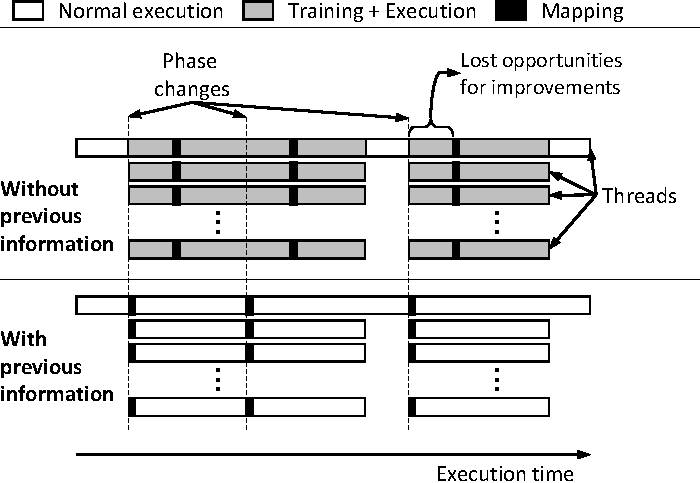
\includegraphics[width=\linewidth]{img/timeline}
%    %!TEX encoding=UTF-8 Unicode
%!TEX root=../tabarnac.tex

\def\len{6}
\def\wid{0.3}
\def\dis{0.1}

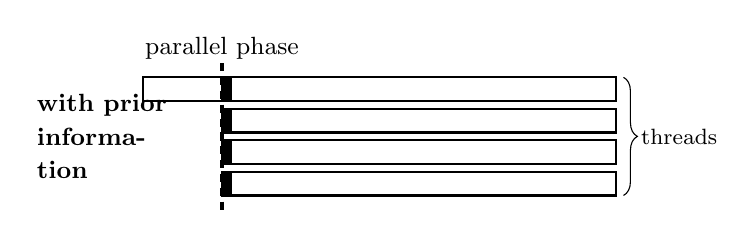
\begin{tikzpicture}
	\node[align=left, text width=1.7cm] at (-0.5,-\wid-1.5*\dis) (label1) {\bfseries\small with prior information};

	\draw[thick] (0,0)              rectangle +(\len, \wid);
	\draw[thick] (1,-\wid*0-\dis*1) rectangle +(\len-1,-\wid);
	\draw[thick] (1,-\wid*1-\dis*2) rectangle +(\len-1,-\wid);
	\draw[thick] (1,-\wid*2-\dis*3) rectangle +(\len-1,-\wid);

	\draw[fill=black] (1,0)              rectangle +(0.12,\wid);
	\draw[fill=black] (1,-\wid*0-\dis*1) rectangle +(0.12,-\wid);
	\draw[fill=black] (1,-\wid*1-\dis*2) rectangle +(0.12,-\wid);
	\draw[fill=black] (1,-\wid*2-\dis*3) rectangle +(0.12,-\wid);

	\draw[very thick,densely dashed] (1,1.6*\wid) -- +(0,-\wid*5-\dis*4.3) node[near start,pos=-0.1] {\small parallel phase};

	\draw [decorate,decoration={brace,amplitude=5pt}] (\len+.1,\wid) -- ++(0,-4*\wid-3*\dis) node [midway,right=1mm]{\footnotesize threads};

	% \draw (-1.35,-\wid*5) -- +(8.8,0); %separator


\end{tikzpicture}


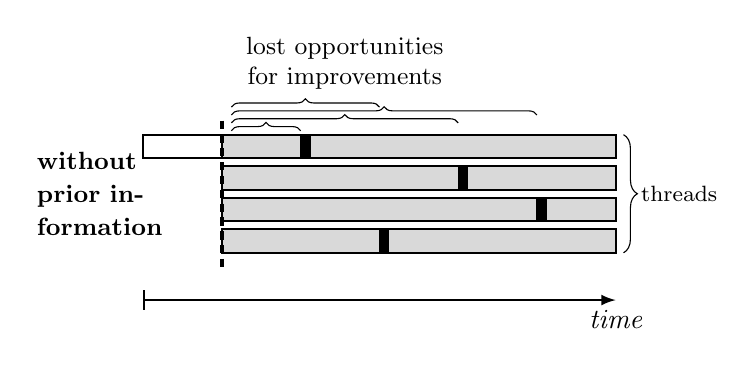
\begin{tikzpicture}
	\node[align=left, text width=2cm] at (-0.35,-\wid-1.5*\dis) (label1) {\bfseries\small without prior information};

	\draw[thick] (0,0)              rectangle +(\len, \wid);
	\draw[fill=gray!30, thick] (1,0)              rectangle +(\len-1, \wid);
	\draw[fill=gray!30, thick] (1,-\wid*0-\dis*1) rectangle +(\len-1,-\wid);
	\draw[fill=gray!30, thick] (1,-\wid*1-\dis*2) rectangle +(\len-1,-\wid);
	\draw[fill=gray!30, thick] (1,-\wid*2-\dis*3) rectangle +(\len-1,-\wid);

	\draw[fill=black] (2,0)              rectangle +(0.12,\wid);
	\draw[fill=black] (4,-\wid*0-\dis*1) rectangle +(0.12,-\wid);
	\draw[fill=black] (5,-\wid*1-\dis*2) rectangle +(0.12,-\wid);
	\draw[fill=black] (3,-\wid*2-\dis*3) rectangle +(0.12,-\wid);

	\draw[decorate,decoration={brace,amplitude=3pt}] (1+0.12,\wid+0.05) -- +(1-0.12,0);
	\draw[decorate,decoration={brace,amplitude=3pt}] (1+0.12,\wid+0.15) -- +(3-0.12,0)node[midway,above=3mm,align=center,font=\small] {\small lost opportunities\\ for improvements};
	\draw[decorate,decoration={brace,amplitude=3pt}] (1+0.12,\wid+0.25) -- +(4-0.12,0);
	\draw[decorate,decoration={brace,amplitude=3pt}] (1+0.12,\wid+0.35) -- +(2-0.12,0);

	\draw[very thick,densely dashed] (1,1.6*\wid) -- +(0,-\wid*5-\dis*4.3);

	\draw[decorate,decoration={brace,amplitude=5pt}] (\len+.1,\wid) -- ++(0,-4*\wid-3*\dis) node [midway,right=1mm]{\footnotesize threads};

	\draw[thick,|-latex] (0,-\wid*6) -- +(\len,0) node[below] {\itshape time};

\end{tikzpicture}

%    \caption{Comparison of data mapping mechanisms with and without prior information about the memory access behavior of a parallel application consisting of four threads. Training is similar to the normal execution, but with additional training overhead.}
%    \label{fig:timeline}
%\end{figure}

%\subsubsection{Mechanisms Without Prior Information}

%Most mechanisms that have no prior information about the memory access behavior operate within the operating system.
On NUMA architectures, data mapping mechanisms have the goal of improving the locality and balance of memory access between NUMA nodes.
Traditionally, operating systems have used the \emph{first-touch}~\cite{Marchetti1995}, \emph{next-touch}~\cite{Lof2005} and \emph{interleave}~\cite{Kleen2004} policies to map memory pages to NUMA nodes.
The first-touch policy, which is the default policy in most operating systems (such as Linux), allocates a page on the NUMA node that performs the first memory access to it.
It requires the developer to take care of which thread accesses data
first, as an incorrect first access can hurt performance.
In next-touch~\cite{Lof2005}, each page is periodically migrated to the NUMA
node that performs the next access to a page. This technique is more flexible than first-touch,
but can lead to excessive page migrations.
The interleave policy (available in Linux via the \texttt{numactl}
tool~\cite{Kleen2004}) distributes memory pages cyclically among all NUMA nodes,
to improve load balance among memory controllers, but it does not take any locality into account.

Newer developments in operating systems focus on refining the data mapping during the execution of parallel applications, using online profiling.
Recent versions of the Linux kernel contain the
NUMA Balancing technique~\cite{Corbet}, which uses page faults to determine if
a page should be migrated to a different NUMA node.%To increase the accuracy
%of this mechanism, extra page faults are inserted at runtime, creating an additional overhead.
%A similar proposal is the AutoNUMA approach~\cite{Corbet2012}.
%Neither mechanism maintains an access history. This eliminates the need to store the access behavior, but also makes them susceptible to excessive migrations.
%Other proposals store such an access history.
%Dashti et al.~\cite{Dashti2013} introduced the Carrefour mechanism, which uses instruction-based sampling~(IBS)~\cite{Drongowski07Instructionbased} available in recent AMD architectures~\cite{AMD2012} to detect the memory access behavior.
%kMAF~\cite{Diener2014} is a similar mechanism that uses page faults to analyze the behavior.
%Due to the access history, these mechanisms can avoid excessive migrations, but still suffer from later migrations and a runtime overhead compared to mechanisms with prior information.
% hardware
% marathe, lapt
%\subsubsection{Mechanisms With Prior Information}
Other solutions improve data mapping in the compiler, the runtime or at a library level.
Piccoli et al.~\cite{Piccoli2014} propose a compiler extension that analyzes
the memory accesses patterns of parallel loops and uses this information to migrate
pages before executing the loop.
%Nikolopoulos et al.~\cite{Nikolopoulos2000a,Nikolopoulos2000} present an integrated compiler/OS-based data mapping mechanism based on a custom OpenMP compiler and IRIX kernel extensions. The compiler inserts instrumentation code to identify access patterns to shared memory areas and to guide migration decisions.
% \DB{Rewrite next sentence}
% ForestGOMP~\cite{Broquedis2010a} requires source code annotations to identify memory access behavior and is limited to the OpenMP library.
% These techniques use predictions about the memory access behavior, which might be dependent on input data and can cause wrong mappings.
%Furthermore, no improvements to the memory access pattern are performed.
% Previous research also uses memory access traces to perform data mapping~\cite{Marathe2010,Bolosky1992}. These can be useful to determine the maximum gains that can be achieved with mapping policies, but are not applicable in general due to their substantial overhead and the fact that the access behavior might change with different input data and different numbers of threads, for instance.


Libraries such as libnuma~\cite{Kleen2004} and MAi~\cite{Ribeiro2009} provide
the ability to allocate data structures on a particular NUMA node, or with an
interleave policy. These techniques can achieve large improvements, but
require a deep understanding of the applications' memory behavior to use them
efficiently.
Our study provides tools to easily understand the memory behavior
and therefore enable the developer to improve performance significantly.

% An evolution of MAi, the Minas framework~\cite{Ribeiro2010}, optionally uses a source code preprocessor to determine data mapping policies for arrays.
%

\subsection{Summary of Related Work}

% We conclude that tools to improve the memory access behavior on NUMA architectures with prior
% information have the highest potential for improvements.
Several studies already provide tools to analyze memory accesses.
These tools usually point out \emph{which} performance issues occur (such as a
high number of cache misses or accesses to remote NUMA nodes), sometimes
\emph{where} they occur (such as information about the structure, function, or
line of code). Some tools helps to correlate these information to
guess \emph{why} an issue is happening. However, no tool directly provides the
reasons \emph{why} such issues occur and \emph{how} to fix them.
Two types of information can help answering this question: which thread is responsible for the first touch (as the default page mapping of most operating systems depends on it), and how different threads access data structures.
This study presents \TABARNAC, a set of tools to explain \emph{why} performance issues
related to memory occur and \emph{how} they can be resolved.

%The two main challenges for this type of tool is to gather information about the memory access patterns in a fast, accurate and easy-to-use way, and providing information to the developers about the ways to improve the behavior of their applications.
%This study, provides a comprehensive solution for these challenges.

% \MD{mechanisms with prior information have highest potential for improvements, but currently:
% - lack of information about memory access behavior
% - lack of information about ways to improve behavior
% }
% Importance of Mapping:
% \begin{itemize}
%     \item First touch
%     \item Interleave
% \end{itemize}

% Why Not automated tools
% \begin{itemize}
%     \item Trainning time
%     \item Garbage in/ garbage out (matrix modulo / bloc)
% \end{itemize}

% New tool: understand why performances are bad
